
%\documentclass[tikz,convert={convertexe={magick.exe}}]{standalone}
\documentclass[tikz,convert]{standalone}
\usetikzlibrary{arrows}

\usepackage{ifthen}

\begin{document}
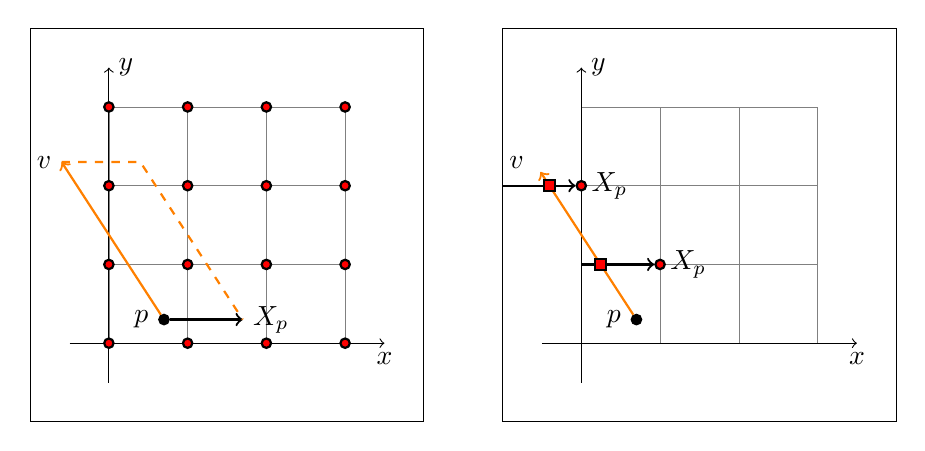
\begin{tikzpicture}

\tikzstyle atom=[circle, draw, inner sep=1.2pt, fill=red, thick]

\begin{scope}

\foreach \x in {0,...,3}
\draw[style=help lines, very thin] (\x,0) -- (\x,3);
\foreach \y in {0,...,3}
\draw[style=help lines, very thin] (0,\y) -- (3,\y);

\draw[->] (-.5,0)--(3.5,0) node[below] {$x$};
\draw[->] (0,-.5)--(0,3.5) node[right] {$y$};

\foreach \x in {0,...,3}
\foreach \y in {0,...,3}
\node[atom] at (\x,\y) {};

\node[atom,fill=black,label=left:$p$] (P) at (.7,.3) {};

\draw[->,thick] (P) -- +(1,0) node[right] {$X_p$};

\draw[->,thick,orange] (P) -- +(-1.3,2) node[left,black] {$v$};

\draw[dashed,orange,thick] (P)++(-1.3,2) -- ++(1,0) -- ++(1.3,-2);

\draw (-1,-1) rectangle (4,4);

\end{scope}


\begin{scope}[xshift=6cm]

\foreach \x in {0,...,3}
\draw[style=help lines, very thin] (\x,0) -- (\x,3);
\foreach \y in {0,...,3}
\draw[style=help lines, very thin] (0,\y) -- (3,\y);

\draw[->] (-.5,0)--(3.5,0) node[below] {$x$};
\draw[->] (0,-.5)--(0,3.5) node[right] {$y$};

\node[atom] (A) at (1,1) {};
\node[atom] (B) at (0,2) {};

\node[atom,fill=black,label=left:$p$] (P) at (.7,.3) {};
\path (P) + (-1.3,2) node[name=PV] {};

\draw[->,thick] (0,1) -- (A) node[right] {$X_p$};
\draw[->,thick] (-1,2) -- (B) node[right] {$X_p$};

\draw[->,thick,orange] (P) -- (PV) node[left,black] {$v$};


\draw (-1,-1) rectangle (4,4);

\node[atom,rectangle,inner sep=2pt] at (intersection of P--PV and 0,1--1,1) {};
\node[atom,rectangle,inner sep=2pt] at (intersection of P--PV and -1,2--0,2) {};

\end{scope}

\end{tikzpicture}
\end{document}